\begin{frame}{The problem}
\small
\begin{columns}
\begin{column}{0.5\textwidth}
\begin{figure}[h!]
    \centering
    
\includegraphics[width=0.8\linewidth]{img/snoots.png} % Replace 'filename.jpg' with your image file
\end{figure}

\vspace{-.5cm}
\end{column}
\begin{column}{0.5\textwidth}
\begin{figure}[h!]
    \centering
    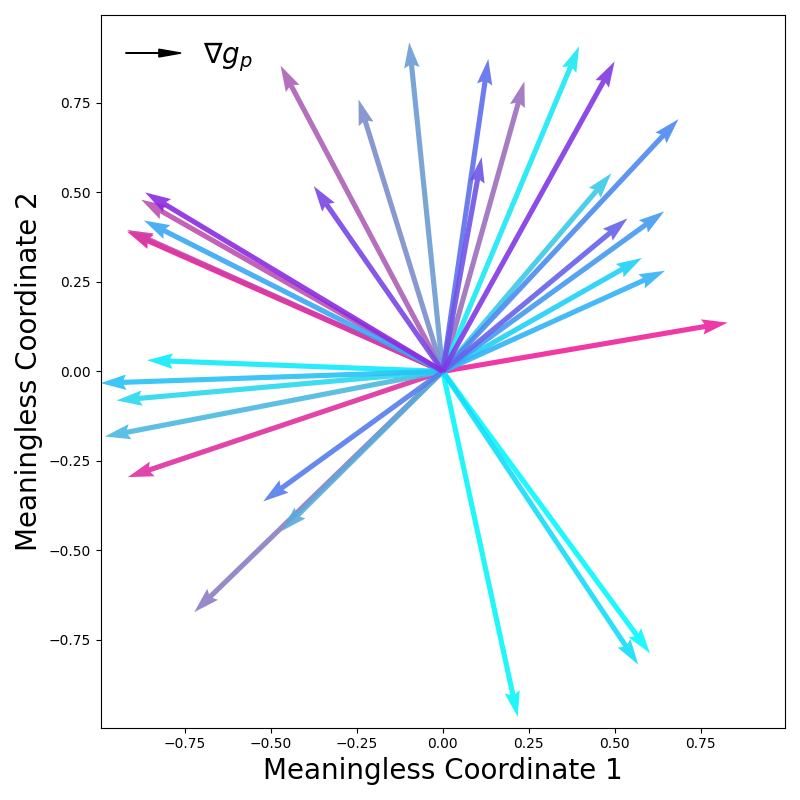
\includegraphics[width=1.\linewidth]{../figures/interpretabledirections.png} % Replace 'filename.jpg' with your image file
\end{figure}
\vspace{-.5cm}
\end{column}
\end{columns}
\end{frame}

\begin{frame}{Isometry selection}
\small

\begin{figure}[h!]
    \centering
    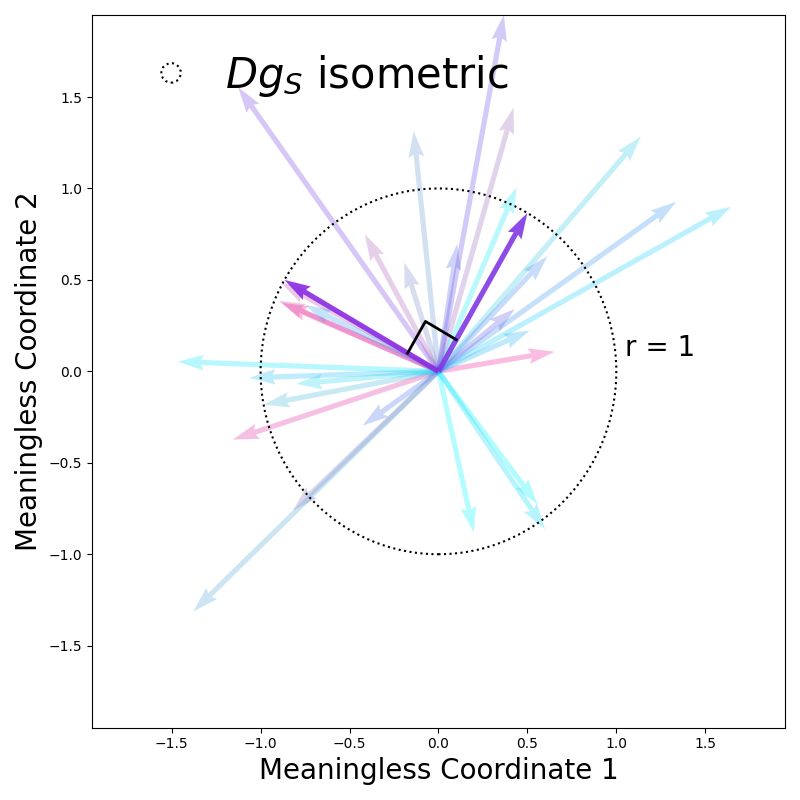
\includegraphics[width=.6\linewidth]{../figures/goldencompass.png} % Replace 'filename.jpg' with your image file
\end{figure}

\end{frame}

\begin{frame}{Yet another matrix loss}
\small
\begin{columns}
\begin{column}{0.5\textwidth}
Given a rank $D$ matrix $X \in \mathbb{R}^{D \times P}$ with singular values $\sigma_d \in [D]$, let
\begin{align*}
\ell_{c}: \mathbb{R}^{D \times P} &\to \mathbb{R}^+ \\
X &\mapsto \sum_{d=1}^D g(\sigma_d(X), c) - D\\
\\[-1ex]
g: \mathbb{R}^+ \times \mathbb{R}^+ &\to \mathbb{R}^+ \\
(t, c) &\mapsto \frac{e^{t^c} + e^{t^{-c}}}{2e}.
\end{align*}
\vspace{-.5cm}
\end{column}
\begin{column}{0.5\textwidth}
\begin{figure}[h!]
    \centering
    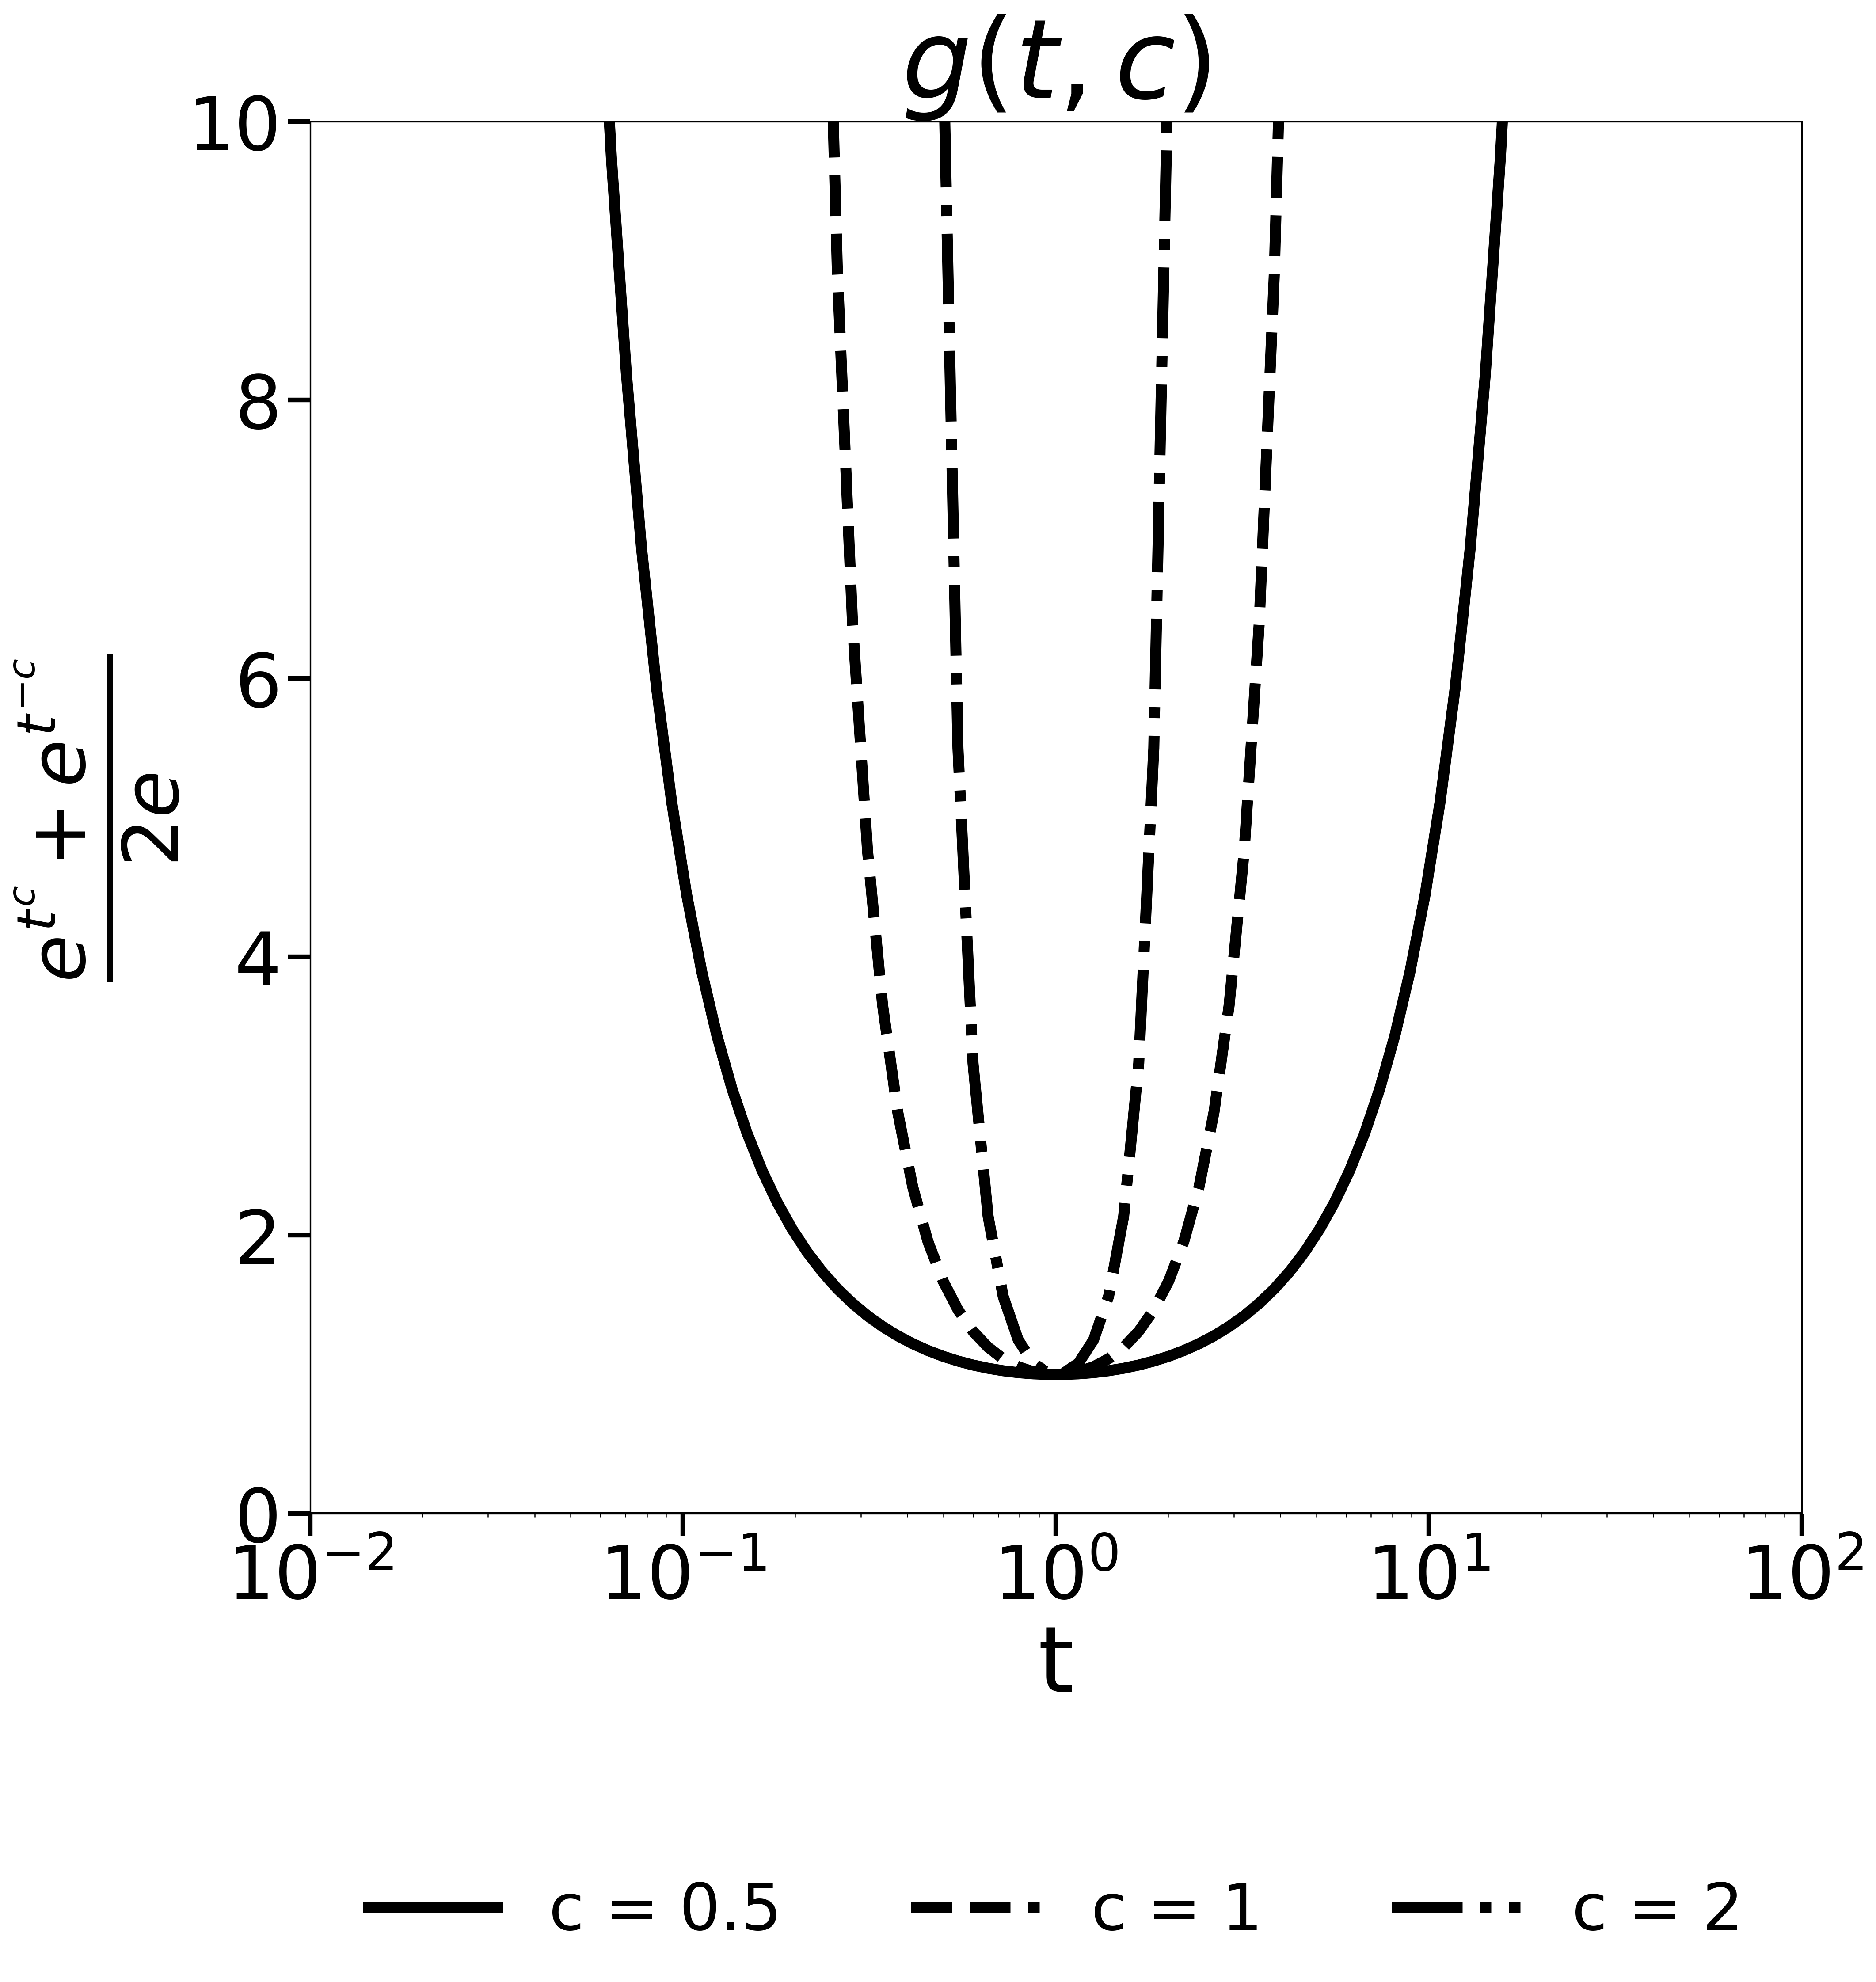
\includegraphics[width=.6\linewidth]{../figures/Figure_1a_ct} % Replace 'filename.jpg' with your image file
\end{figure}
\begin{figure}[h!]
    \centering
    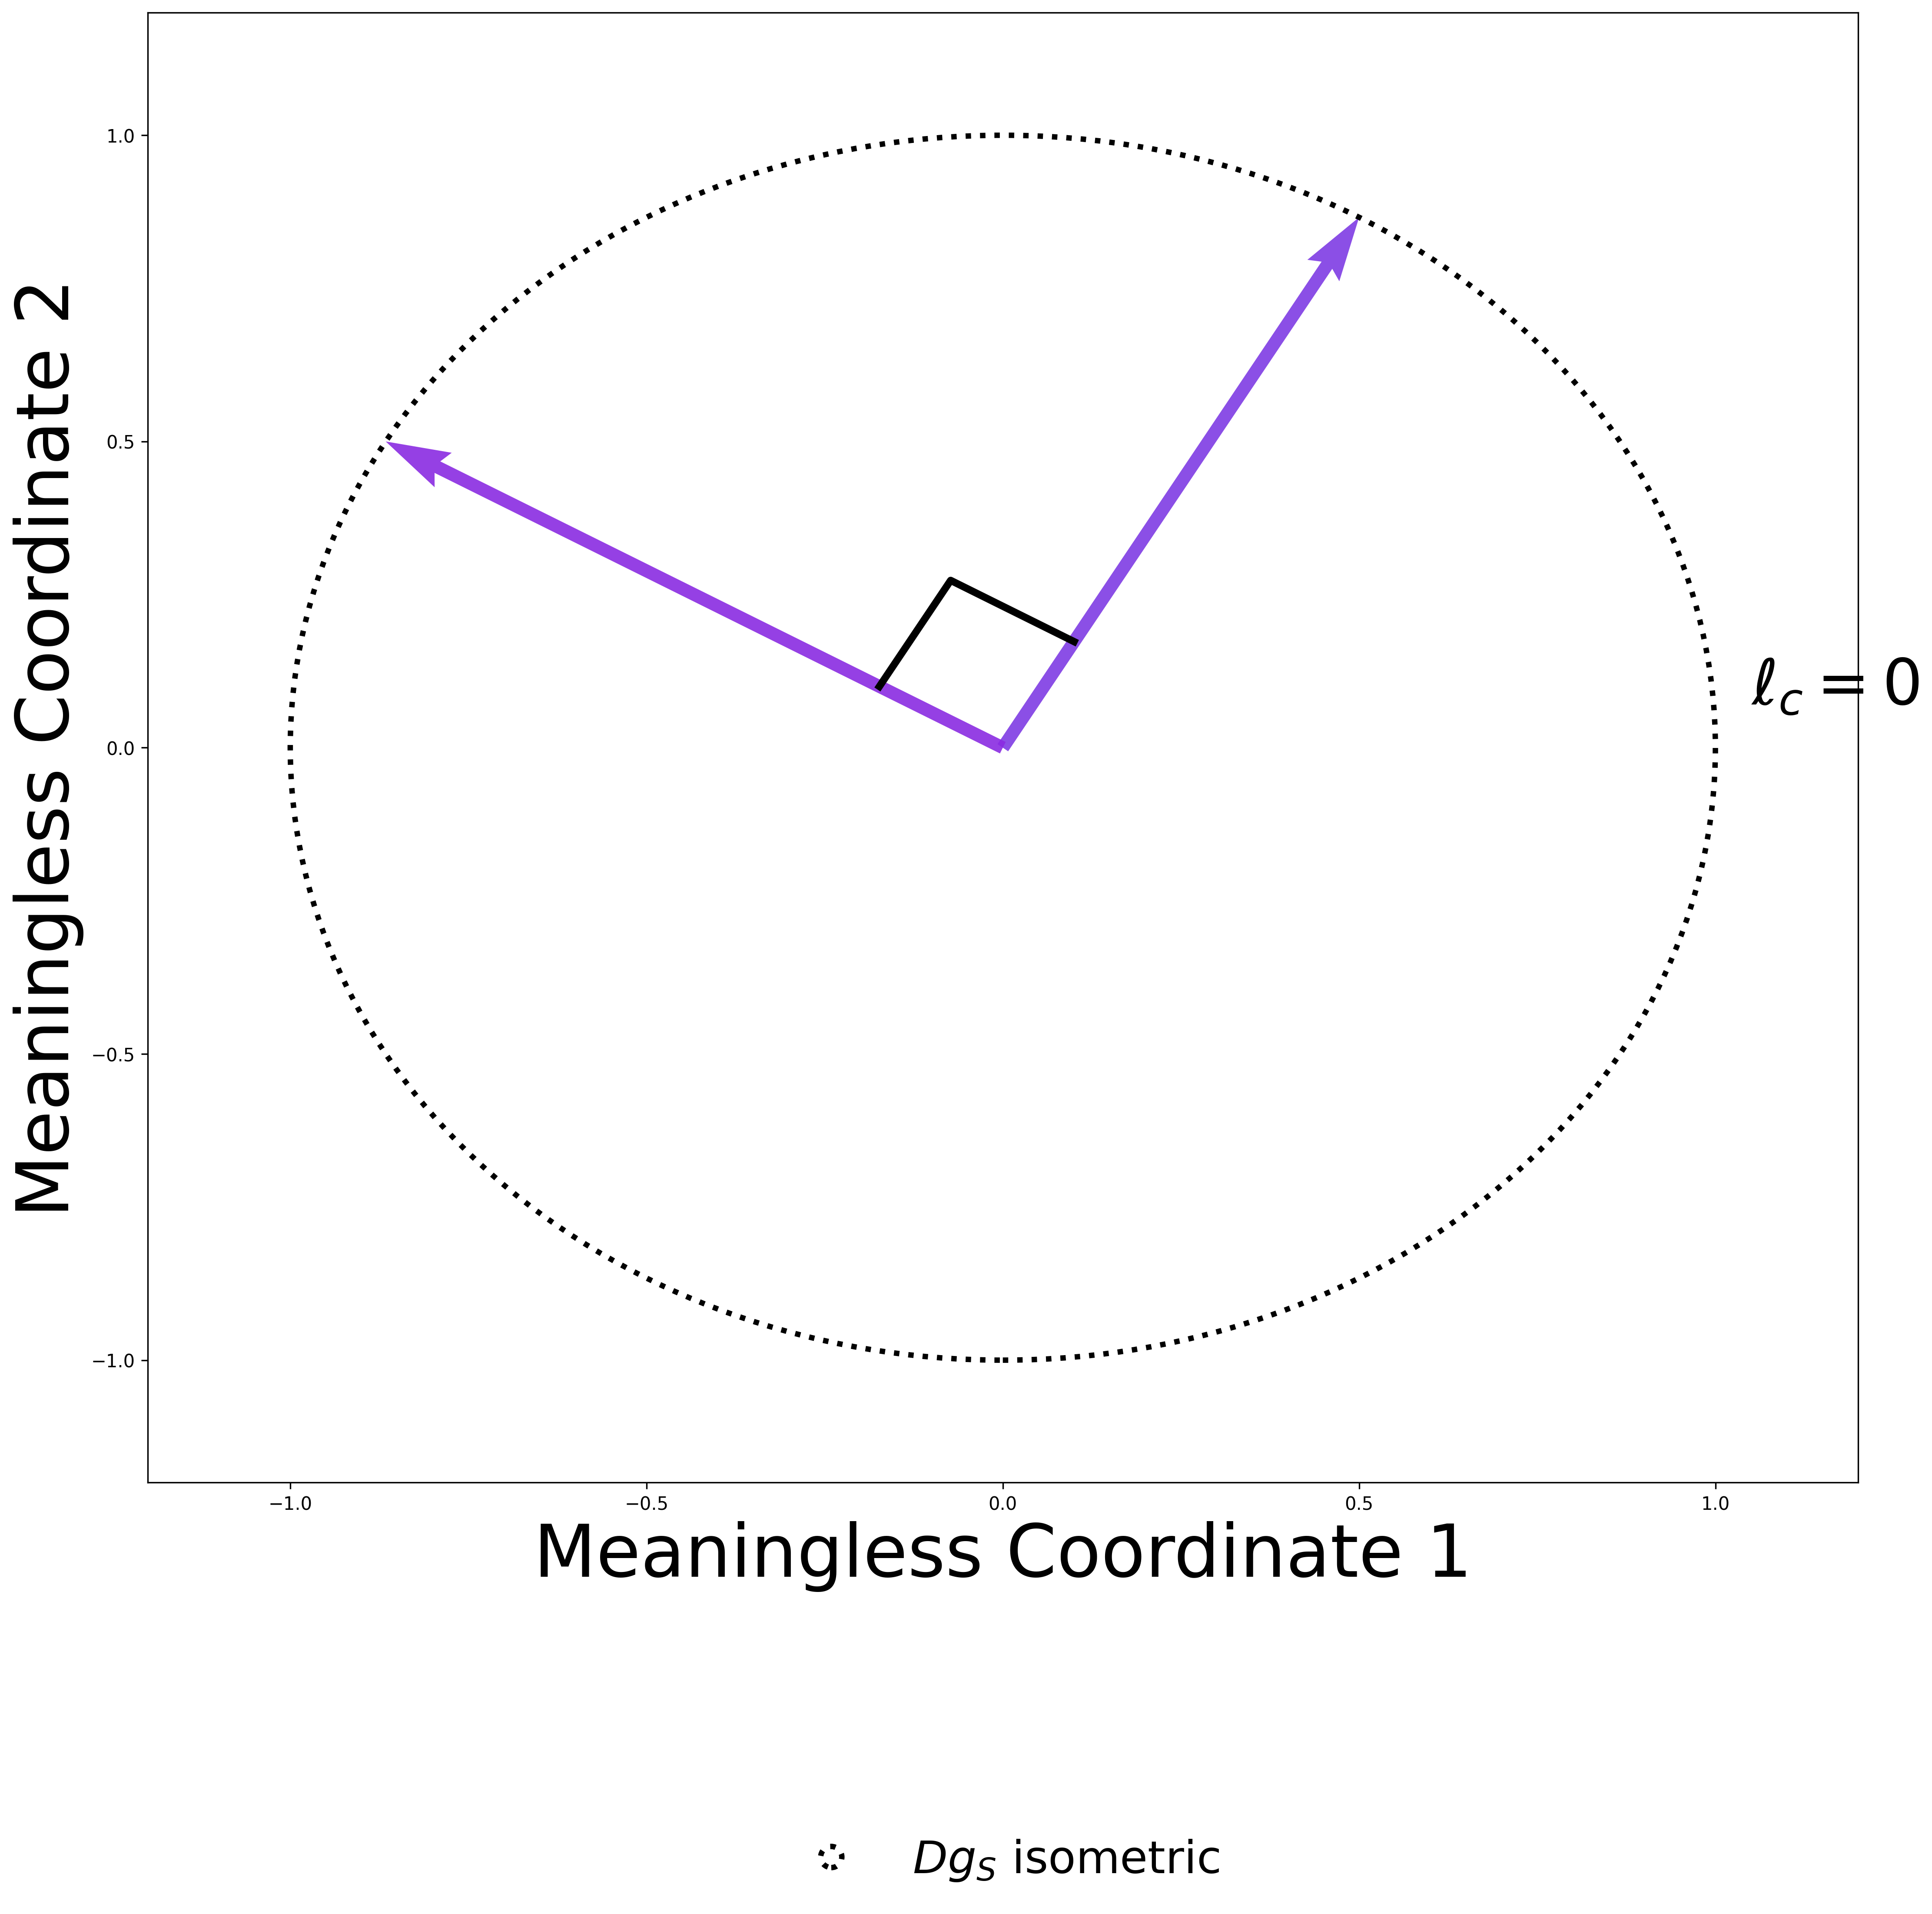
\includegraphics[width=.6\linewidth]{../figures/isometree} % Replace 'filename.jpg' with your image file
\end{figure}
\end{column}
\end{columns}
\end{frame}



